%!TEX root = paper.tex
\begin{figure}[h]
  \centering
  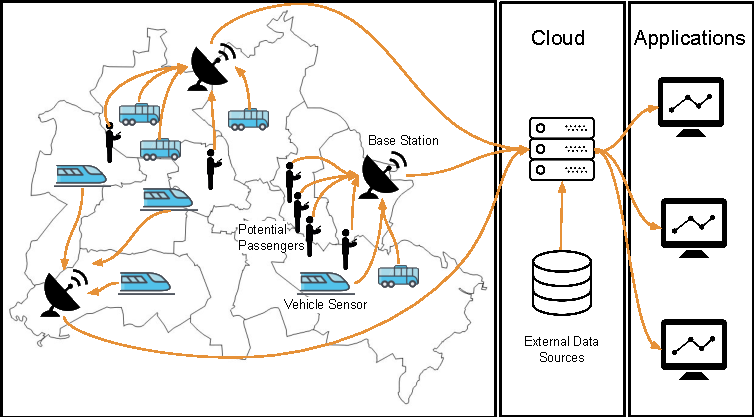
\includegraphics[width=\linewidth]{figs/iot_scenario}
  \caption{Common IoT Infrastructure.}
  \label{fig:iot-app-scenario}
\end{figure}
\section{Data Management in the IoT}
\label{iot}
% 
% In this section, we discuss present our demonstrated IoT use case and point out why state of the art cloud-based SPEs fall short to address those.
% 
% \subsection{Public Transport as an IoT Scenario}
Today's data management application scenarios in the IoT cover a broad range, e.g., failure prediction and anomaly detection in factories, training models for self-driving cars, or tracking of supply chains. 
In the following, we present a representative IoT scenario, and describe the challenges associated with query processing.
In general, IoT scenarios comprise of moving or static sensors connected to the cloud through multiple intermediate nodes.

\subsection{IoT Application Scenarios}
In \Cref{fig:iot-app-scenario}, we show a public transport system as a representative IoT application. 
In this system, vehicles and potential public transport passengers with attached sensors move around the city.
Sensors transmit their data in regular time intervals to geographically distributed base stations, which forward sensor data to the cloud. 
The base stations, as well as the vehicles, represent intermediate nodes in the IoT infrastructure.
On the cloud, sensor streams are subject to enrichment from external sources, e.g., weather or air pollution data.
The resulting data streams are then fed into applications, to answer ad-hoc user queries, to visualize data in GUIs, or to perform advanced analytics.
If a city would implement such an IoT infrastructure, it would enable smart city optimizations such as:
\begin{itemize} 
	\item Reduce air pollution by traffic light control mechanisms.
	\item Ad-hoc route planning to cope with sudden traffic jams.
	\item Automate schedule updates for the public transport based on crowdedness.
\end{itemize}
\textcolor{red}{Laura: Was machen wir an dieser Stelle mit Prof. Markls feedback?}
% 
% \subsection{Fast Decision Taking}
% Datasets of collected sensor data can either be processed in a static or in a dynamic way. 
% In IoT scenarios, it does not always make sense to store all sensor data and perform analytics on outdated static datasets. 
% In contrast, it is of great value to be able to analyze data in real time, and to react to detected patterns, either automatically or with human intervention. For example, when detecting areas with high demand or vehicle failures, it is necessary for an employee to schedule new vehicles.
% \textcolor{red}{(@TODO,der Absatz macht für mich keine Sinn, würde ihn rausnehmen, was willst du denn hier sagen?)}

\subsection{IoT Infrastructure Challenges}
In the following, we discuss challenges related to data management in the IoT. 
Zeuch et al. \cite{nes} point out, that cloud-based SPEs rely on assumptions that IoT infrastractures violate.
First, both paradigms introduce different network topologies.
In particular, processing nodes in cloud-based SPEs are densely connected, i.e., each node can communicate with all other nodes.
In contrast, IoT infrastructures follow a structure similar to p2p networks, where the physical network topology predefines the paths from data sources (sensors) to data sinks (cloud). 
Therefore, every node accesses only a subset of data routed through it. 
For example, a base station located in the west of a city is not able to directly access sensor streams that sensors generate in the east of said city. 
In today's IoT infrastructures, there are orders of magnitude more sensors than nodes. Hence, this physical setup forms a tree-like graph where data flows from sensors among the intermediate nodes to a sink in the cloud.
Finally, when considering multiple layers of intermediate nodes, there might be multiple paths from the source to the cloud. 
Second, both paradigms expect differently sized input streams.
In the fog infrastructure, millions of sensors constantly produce small data streams that capture physical phenomena, such as earthquakes. 
In contrast, cloud-based SPEs are built around the assumptions that few, large data streams, or utilized data brokers (e.g., Kafka) produce them as an input. \textcolor{red}{Laura: Produce what as an input? Bleibt leider auch bei mehrmaligem Lesen unklar.}
% Intermediate nodes are used to transfer data from sensors to the cloud.
% Thus, intermediate nodes are part of the physical environment, e.g., mobile phones, base stations, routers, system-on-a-chip devices, or even regular servers.
%In contrast to robust cloud network infrastructures, network connections in the IoT range from high-speed Ethernet connections to unstable LoWPAN networks and Bluetooth connections. 
%Additionally, nodes constantly change their geospatial location and might cause transient failures, e.g., a bus driving through a tunnel.
% 
%\textbf{Optimizing Across Queries and Operators.}
%IoT applications support two major types of queries, long-running and ad-hoc. 
%Modern SPEs scale-out computation for a large number of queries. However, they only possess minor capabilities to optimize across queries, e.g., when sharing a set of common predicates. 
%Furthermore, some queries have to handle a state (intermediate results) of considerable size, e.g., for window aggregations. 
%However, intermediate IoT nodes provide commonly only restricted storage capabilities.
%This problem is magnified when scaling the number of queries. 
%Therefore, it is necessary for IoT data management platforms to employ data sharing techniques both among queries and operators, techniques proposed by AStream \cite{astream} and Scotty \cite{scotty}.
%\textcolor{red}{(@TODO,mir ist nich ganz klar, sind das denn jetzt die Punkte die du in deiner Demo addressieren willst?)}
